\section{双标记侧寻找$\LtoXiK$~和~$\LtoXisK$}
为了获取双标记事例,我们在先重建一个单侧$\lambdacp$($\lambdacm$)的基础上,再在剩余的径迹中去寻找另外一个$\lambdacm$($\lambdacp$)的候选事例。
为了得到$\LtoXiK$~和~$\LtoXisK$的候选态,
我们要求单标记侧的$\lambdacp$($\lambdacm$)的$M_{\rm BC}$应该落在信号区$(2.282,2.291)\gevcc$内。
同时我们再找一条额外的带电径迹($\Xi^{0}$和$\Xi{(1530)}^{0}$不去重建),其电荷号应该要与标记侧$\Lambda_c$的电荷号相反。
接下来我们要求这条带电径迹应该满足$K$介子的粒子鉴别条件,详情如下:
 \begin{itemize}
 \item $|\delta r|<1\,\unit{cm}$, $|\delta z|<10\,\unit{cm}$, $|\cos\theta|<0.93$
 \item  prob($K$)$>$0$\mathcal{\&\&}$prob($K$)$>$prob($\pi$)
 \end{itemize}
双标记事例寻找过程中如果有了多个$K$介子候选者,我们会保留所有的候选者。
在数据目前的统计量下,我们没有发现有同一个事例进来多个候选者的情况(多重数)。
我们用大量的MC样本对多重数比例进行研究发现这个比例只有0.1\%,这一比例在目前的测量精度下,完全可以安全地忽略。

为了鉴别$\LtoXiK$~和~$\LtoXisK$的信号,我们利用变量$M_{\rm miss}$来抽取信号。
其定义为:
\begin{equation}
M_{\rm miss} = \sqrt{E_{\rm miss}^{2}-|\overrightarrow{p}_{\rm miss}|^{2}}
\end{equation}
其中,$E_{\rm miss}$和$\overrightarrow{p}_{\rm miss}$是丢失的,没有重建的$\Xi^{0}$和$\Xi{(1530)}^{0}$的能量和动量。
$E_{\rm miss}$用如下公式计算,
\begin{equation}
E_{\rm miss} = E_{\rm beam}-E_{\rm K^{+}}
\end{equation}
其中$E_{\rm beam}$ 指的是束流能量, $E_{\rm K^{+}}$ 是 $K^{+}$介子在$\ee$质心系内的测量能量。
变量$\overrightarrow{p}_{\rm miss}$ 的计算通过
\begin{equation}
\overrightarrow{p}_{\rm miss} = \overrightarrow{p}_{\lambdacp} - \overrightarrow{p}_{\rm K^{+}}
\end{equation}
其中$\overrightarrow{p}_{\lambdacp}$ 和 $\overrightarrow{p}_{\rm K^{+}}$ 分别是 $\lambdacp$ 和 $K^{+}$ 的动量。
$\lambdacp$的动量计算通过如下公式,
\begin{equation}
\overrightarrow{p}_{\lambdacp}  = -\hat{p}_{\rm tag}\cdot\sqrt{E_{\rm beam}^{2}-m_{\lambdacp}^{2}}
\end{equation}
其中 $\hat{p}_{\rm tag}$ 是单标记侧$\lambdacm$的单位动量方向,$m_{\lambdacp}$ 是PDG2016~\cite{PDG2017}收录的$\lambdacp$质量。
如果我们找到的$K^{+}$介子是来自$\Lambda_{c}^{+}\to \Xi^{0(*)}K^{+}$过程,则其在$M_{\rm miss}$谱上会在$1.31486\gevcc$或者$1.5318\gevcc$附近出现峰状结构,这两个结构就对应着$\Xi^{0}$ 和 $\Xi{(1530)}^{0}$。

我们将12个单标记道对应的双标记产额加在一起来处理,并且合并电荷共轭的道以此来估计公式\ref{eq:br}中的$N_{-,\XiXisK}^{DT}$。
如图~\ref{fig:DT_data}所示为合并了12个单标记道的$M_{\rm miss}$分布,其中红色的直方图为落在单标记侧$\lambdacm$ $M_{\rm BC}$在信号区$(2.282, 2.291)\gevcc$范围内的事例。
相应的,蓝颜色直方图为单标记侧$\lambdacm$ $M_{\rm BC}$在边带区$(2.25, 2.265)\gevcc$内的事例分布。
我们可以清楚的看到$\Xi^{0}$ 和 $\Xi{(1530)}^{0}$的信号峰,同时在信号区域,边带区事例不会贡献峰状本底。
此外,我们也用\textbf{Cocktail MC}样本来检查是否存在其它一些可能的峰状本底。
其$M_{\rm miss}$的分布见图~\ref{fig:DT_mc},我们可以注意到并没有峰状本底的贡献。

\begin{figure*}[hp]
\centering
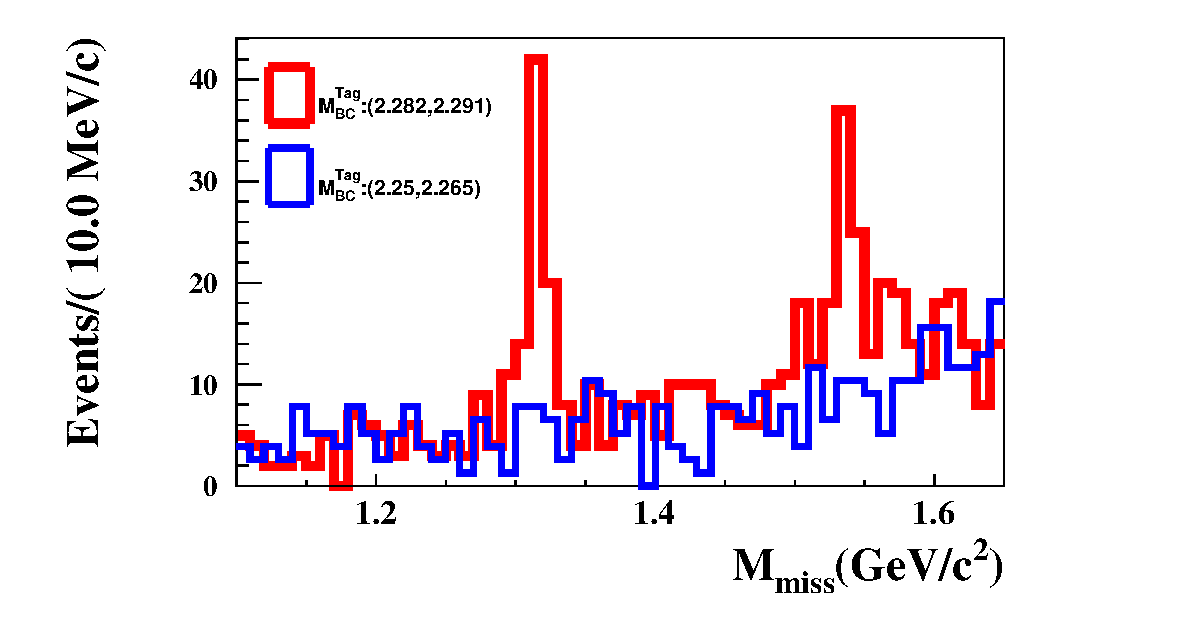
\includegraphics[width=0.9\textwidth]{chap2_MissingMass}
\caption{双标记侧\textbf{data}的$M_{\rm miss}$的分布。红色直方图对应单标记侧$\lambdacm$ $M_{\rm BC}$在信号区$(2.282, 2.291)\gevcc$的分布。 蓝色直方图对应边带区$(2.25, 2.265)\gevcc$的事例。}
\label{fig:DT_data}


\end{figure*}
\begin{figure*}[hp]
\centering
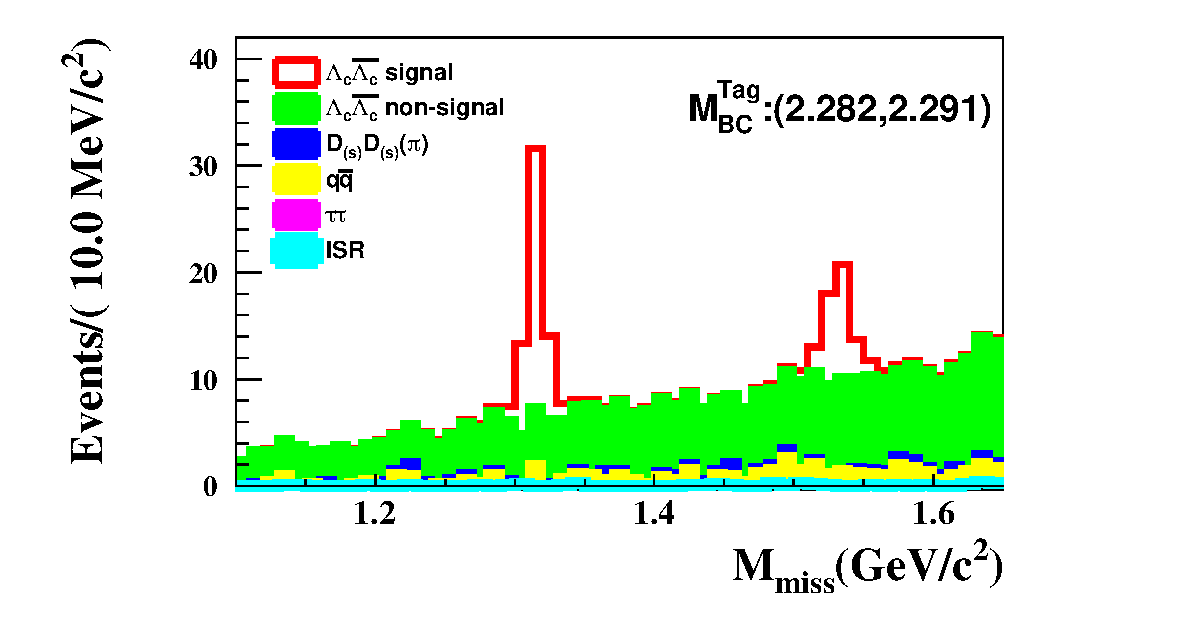
\includegraphics[width=0.9\textwidth]{chap2_MissingMass_bkg}
\caption{双标记侧\textbf{Cocktail MC}的$M_{\rm miss}$分布.}
\label{fig:DT_mc}
\end{figure*}

\section{双标记数据分析}

我们采用不分区间的最大似然拟合来抽取$\LtoXiK$~和~$\LtoXisK$的信号数目。
图~\ref{fig:DT_datafit}给出了双标记侧$M_{\rm miss}$的拟合结果图。
拟合函数中都包含着两部分,信号形状和本底形状。
信号形状我们采用来自于双标记MC的信号形状卷积一个高斯函数来描述。
这里高斯的参数是浮动的。
图中黑色的带误差的点是数据,红线是总的拟合线,
本底用二阶多项式函数来描述。
拟合给出的$\XiK$和$\XisK$的产额分别为$N_{-,\XiK}=68.2\pm9.9$和$N_{-,\XisK}=59.5\pm11.7$。
通过比较放信号与不放信号拟合两种情况下拟合的似然值的变化,我们可以得出两个道的统计显著性,$\Xi^0K^+$为$10.3\sigma$,$\Xi^{*0}K^+$为$6.4\sigma$。
详细的拟合参数值及其各参数之间的关联系数见表~\ref{tab:par}和表~\ref{tab:rho}。

%%%%%%%%%%%%%%%%%%%%%%%%%%%%%%%%%%%%%%%%%%%%%%%%%%%%%%%%%%%%%%%%%%%%%%%%%%%%%%%%%%%%%%%%%
\begin{figure*}[]
\centering
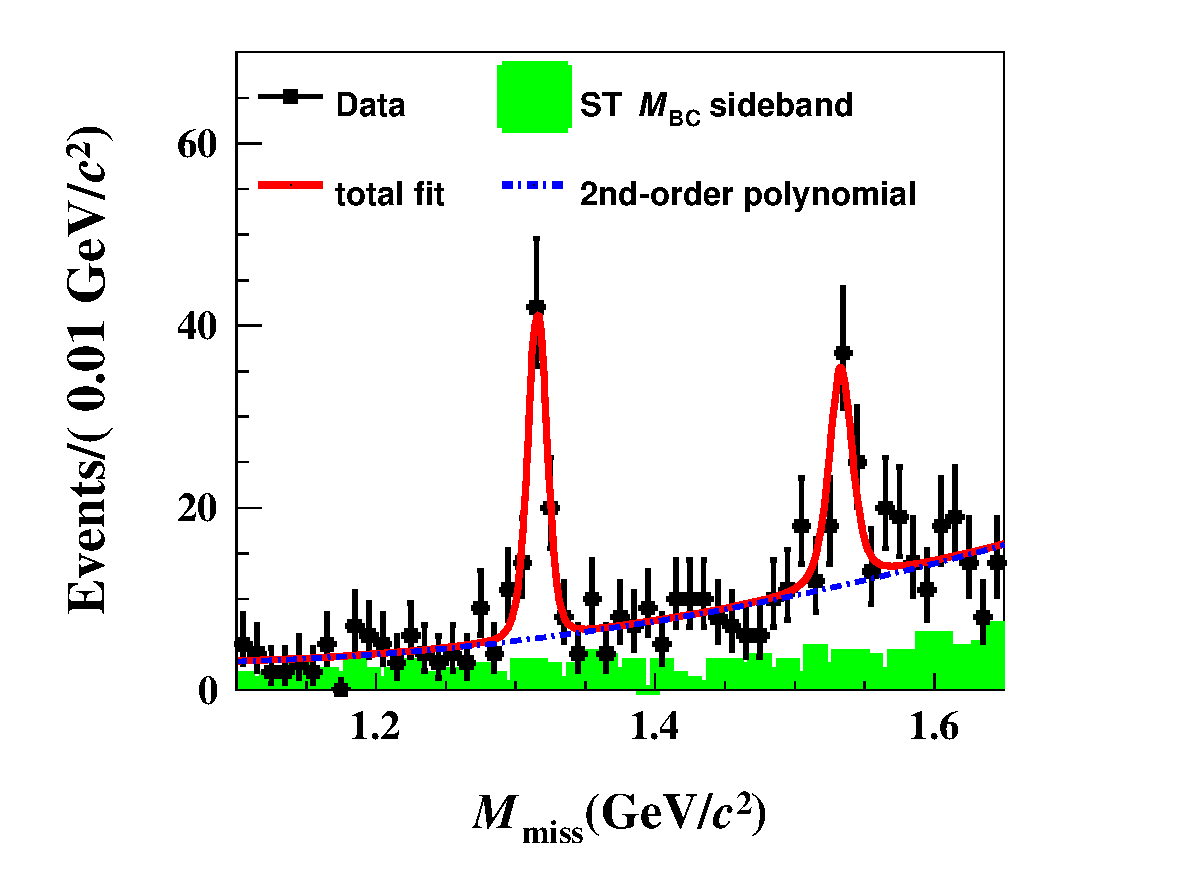
\includegraphics[width=0.9\textwidth]{chap2_fit_MissingMass}
\caption{拟合\textbf{数据}中双标记侧~$M_{\rm miss}$分布得产额的拟合结果图,合并了多个单标记道且包含了电荷共轭的道。在每个图中,黑色的带误差的点代表数据的分布,红色实的曲线是拟合结果,蓝色虚线是二阶多项式函数。}
\label{fig:DT_datafit}
\end{figure*}

\begin{table}[hp]
  \begin{center}
%  \footnotesize
   \caption{数据中 $M_{\rm miss}$ 拟合的参数值。}
  \begin{tabular}{l|c}
      \hline 
参数  & 拟合值及其误差 \\ \hline
$c_{0}$  & $342.3\pm83.9$  \\
$c_{1}$  & $-609.8\pm133.3$  \\
$c_{2}$  & $293.8\pm74.3$  \\
$N_{bkg}$  & $429.3\pm23.2$  \\
$N_{\XiK}$  & $68.2\pm9.9$  \\
$N_{\XisK}$  & $59.5\pm11.7$  \\
$\sigma$  & $0.0015\pm0.0187$  \\
$\mu$  &  $0.0048\pm0.0074$  \\
\hline
   \end{tabular}
   \label{tab:par}
  \end{center}
  \end{table}

\begin{table}[hp]
  \begin{center}
%  \footnotesize
   \caption{数据中 $M_{\rm miss}$ 拟合的参数值之间的关联系数。}
  \begin{tabular}{l|cccccccc}
      \hline 
parameters  &  $c_{0}$   &  $c_{1}$   & $c_{2}$   & $N_{bkg}$  &   $N_{\XiK}$  &  $N_{\XisK}$  &   $\sigma$ &  $\mu$ \\ \hline
$c_{0}$         &   $ 1.000$  &  $-0.889$  &  $ 0.501$  &  $-0.027$  &  $ 0.071$  &  $-0.006$  &  $-0.001$  &  $-0.001$ \\ 
$c_{1}$         &   $-0.889$  &  $ 1.000$  &  $-0.839$  &  $ 0.001$  &  $-0.007$  &  $ 0.004$  &  $ 0.000$  &  $ 0.000$ \\ 
$c_{2}$         &   $ 0.501$  &  $-0.839$  &  $ 1.000$  &  $ 0.026$  &  $-0.080$  &  $ 0.017$  &  $ 0.001$  &  $ 0.001$ \\ 
$N_{bkg}$       &   $-0.027$  &  $ 0.001$  &  $ 0.026$  &  $ 1.000$  &  $-0.139$  &  $-0.293$  &  $ 0.003$  &  $-0.004$ \\ 
$N_{\XiK}$      &   $ 0.071$  &  $-0.007$  &  $-0.080$  &  $-0.139$  &  $ 1.000$  &  $ 0.019$  &  $-0.004$  &  $-0.002$ \\ 
$N_{\XisK}$     &   $-0.006$  &  $ 0.004$  &  $ 0.017$  &  $-0.293$  &  $ 0.019$  &  $ 1.000$  &  $-0.002$  &  $ 0.009$ \\ 
$\sigma$        &   $-0.001$  &  $ 0.000$  &  $ 0.001$  &  $ 0.003$  &  $-0.004$  &  $-0.002$  &  $ 1.000$  &  $ 0.997$ \\ 
$\mu$           &   $-0.001$  &  $ 0.000$  &  $ 0.001$  &  $-0.004$  &  $-0.002$  &  $ 0.009$  &  $ 0.997$  &  $ 1.000$ \\    
\hline
   \end{tabular}
   \label{tab:rho}
  \end{center}
  \end{table}





%和单标记侧类似,我们也对双标记MC样本按照单标记侧的分辨参数对现有MC进行修正。
%然后用这份修正之后的双标记MC样本采用数数的方式去计算电荷共轭的双标记选择效率$\varepsilon_{i^+j^-}^{DT}$~和~$\varepsilon_{i^-j^+}^{DT}$。
%将电荷共轭的双标记过程所得效率进行平均作为最终的双标记选择效率$\varepsilon_{ij}^{DT}$。
%这些效率值是不包含表~\ref{tab:interDecay}中的次级衰变分支比的。
%作为中间计算需要用到的数据,因其篇幅较大暂不予以全部列出$\varepsilon_{ij}^{DT}$,但我们给出按照公式\ref{eq:dteff}计算的约化效率$\varepsilon_{-j}^{\rm DT}$。
%具体见表~\ref{tab:DTyields}。

